\section{Condition initiale}
Les relations nous permettant d'apporter des conditions satisfaisantes au système sont données par les formules de Frank, King et Raine avec $P = P_{gaz}$ et $\kappa_{ff} \gg \kappa_{e}$ \cite{F_K_R-1985}. Ces conditions en $\Sigma$ et $T$ sont suffisamment petites pour ne pas influencer le système lors de son évolution. $\dot{M}$ est pris très petit devant  le taux $\dot{M_{0}}$ imposé au système : 
\begin{equation}
	\dot{M} = 1.10^{-1 }\dot{M_{0}}
\end{equation} 

\begin{equation}
	T = 1.4 \times 10^{4} \alpha^{- \frac{1}{5}} \left[ \frac{\dot{M}}{10^{16} \mbox{g} \mbox{s}^{-1}} \right]^{\frac{3}{10}} \left[ \frac{M}{M_{sol}}\right]^{\frac{1}{4}} \left[ \frac{r}{10^{10} cm}\right]^{- \frac{3}{4}} f^{\frac{3}{10}} \mbox{K} 
\end{equation}

\begin{align}
	\Sigma = 5.2 \alpha^{- \frac{4}{5}} \left[ \frac{\dot{M}}{10^{16} \mbox{g} \mbox{s}^{-1}} \right]^{\frac{7}{10}} \left[ \frac{M}{M_{sol}}\right]^{\frac{1}{4}} \left[ \frac{r}{10^{10} cm}\right]^{- \frac{3}{4}} f^{\frac{7}{10}} \mbox{K}  \\ 
	\text{avec } f = \left[ 1 - \left( \frac{r}{3 r_{s}}\right)^{- \frac{1}{2}}\right]
\end{align}

 \begin{figure}[ht]
   \begin{minipage}[c]{.46\linewidth}
      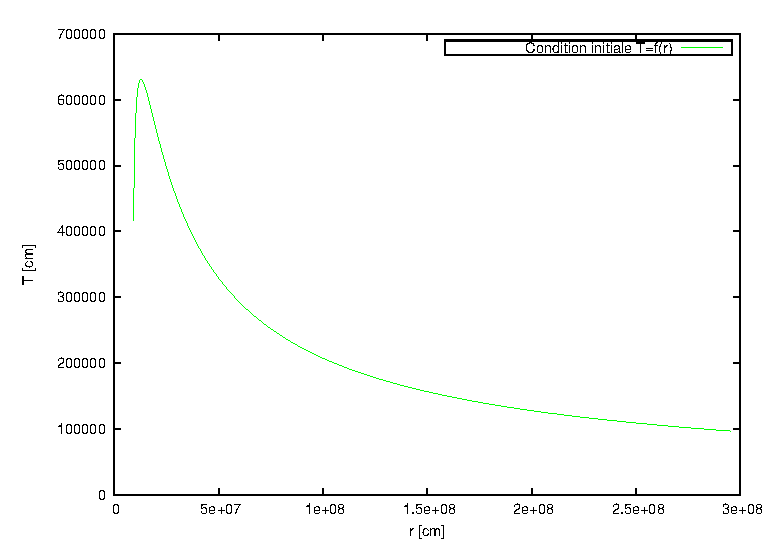
\includegraphics[scale=0.6]{ic_T.eps}
      \caption{Evolution de T en fonction de r à t = 0}\label{fig:CI_T}
   \end{minipage} \hfill
   \begin{minipage}[c]{.46\linewidth}
      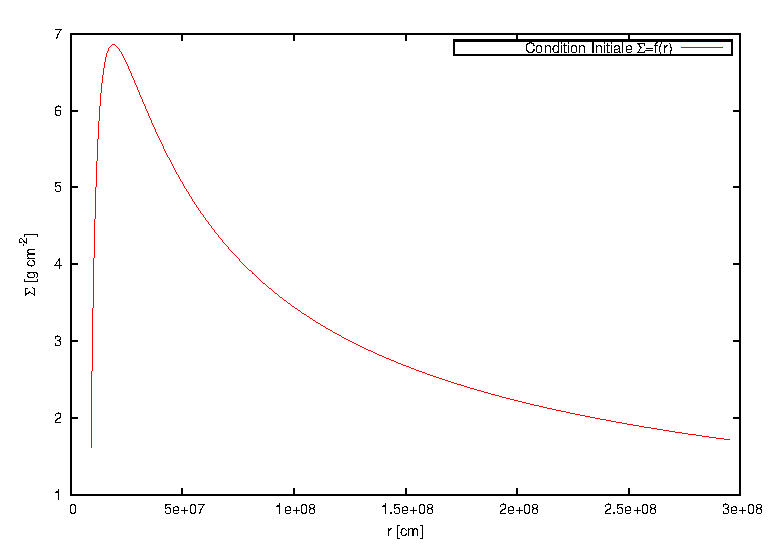
\includegraphics[scale=0.6]{ic_Sig.eps}
      \caption{Evolution de $\Sigma$ en fonction de r à t = 0}\label{fig:CI_Sig}
   \end{minipage}
\end{figure} 


Nous pouvons voir sur les figures \ref{fig:CI_T} et \ref{fig:CI_Sig} les calculs de $T$ et $\Sigma$ en fonction de $r$ à l'instant t = 0 de la simulation. \\


Cela nous permet donc, à partir de l'utilisation du trinôme du second degré explicité équation \eqref{eq:trinôme} de calculer la hauteur du disque à l'instant $t = 0$ du système. \\

Dans le cas limite où s'expriment ces formules nous pouvons également calculer le rapport $H/r$ à partir de la formule suivante : 

\begin{equation}
	\frac{H}{r} = 1.7 \times 10^{-2}\alpha^{- \frac{1}{10}} \left[ \frac{\dot{M}}{10^{16} \mbox{g} \mbox{s}^{-1}} \right]^{\frac{3}{20}} \left[ \frac{M}{M_{sol}}\right]^{- \frac{3}{8}} \left[ \frac{r}{10^{10} cm}\right]^{- \frac{1}{8}} f^{\frac{3}{5}}
\end{equation}
 
Cela nous permet de comparer cette approximation de $H$ à la résolution par trinôme pour ces approximations de $T$ et $\Sigma$ à t = 0. \\

\begin{center}
	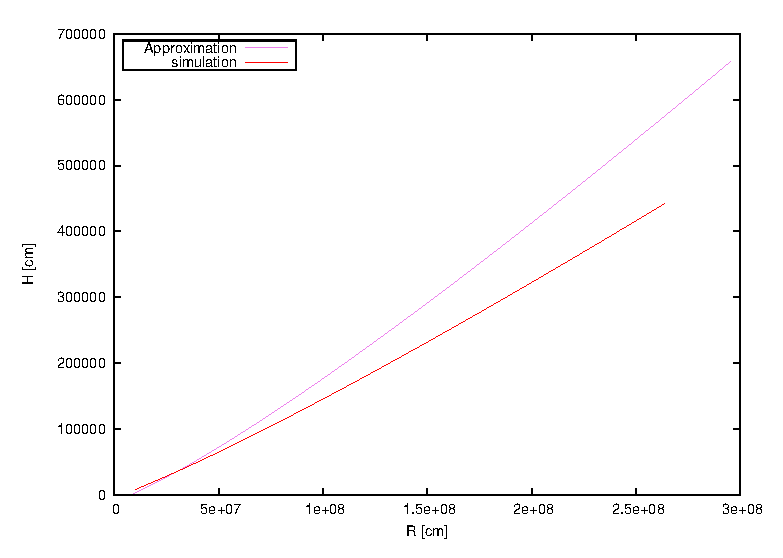
\includegraphics[scale=0.8]{ic_h.eps}
\end{center} 

La forme de notre disque d'accrétion découlant de ces conditions initiales est réaliste compte tenu de la masse du trou noir et de son taux d'accrétion.
